\let\negmedspace\undefined
\let\negthickspace\undefined
\documentclass[journal]{IEEEtran}
\usepackage[a5paper, margin=10mm, onecolumn]{geometry}
%\usepackage{lmodern} % Ensure lmodern is loaded for pdflatex
\usepackage{tfrupee} % Include tfrupee package

\setlength{\headheight}{1cm} % Set the height of the header box
\setlength{\headsep}{0mm}     % Set the distance between the header box and the top of the text

\usepackage{gvv-book}
\usepackage{gvv}
\usepackage{cite}
\usepackage{amsmath,amssymb,amsfonts,amsthm}
\usepackage{algorithmic}
\usepackage{graphicx}
\usepackage{textcomp}
\usepackage{xcolor}
\usepackage{txfonts}
\usepackage{listings}
\usepackage{enumitem}
\usepackage{mathtools}
\usepackage{gensymb}
\usepackage{comment}
\usepackage[breaklinks=true]{hyperref}
\usepackage{tkz-euclide} 
\usepackage{listings}
% \usepackage{gvv}                                        
\def\inputGnumericTable{}                                 
\usepackage[latin1]{inputenc}                                
\usepackage{color}                                            
\usepackage{array}                                            
\usepackage{longtable}                                       
\usepackage{calc}                                             
\usepackage{multirow}                                         
\usepackage{hhline}                                           
\usepackage{ifthen}                                           
\usepackage{lscape}
\begin{document}

\bibliographystyle{IEEEtran}
\vspace{3cm}

\title{6.5.3.1}
\author{EE24BTECH11001 - Aditya Tripathy}
 \maketitle
% \newpage
% \bigskip
{\let\newpage\relax\maketitle}

\renewcommand{\thefigure}{\theenumi}
\renewcommand{\thetable}{\theenumi}
\setlength{\intextsep}{10pt} % Space between text and floats


\numberwithin{equation}{enumi}
\numberwithin{figure}{enumi}
\renewcommand{\thetable}{\theenumi}


\textbf{Question}:\\
Find the local minimum/maximum of the given function:\\
$f\brak{x} = x^2$
\\
\textbf{Solution: }\\
We use the method of gradient descent to find the minimum/maximum of the given function, since the objective function is convex.
Since the coefficient of $x^2 > 0$, we expect to find a local minimum.
\begin{align}
    x_{n+1} &= x_n - \mu f^{\prime}\brak{x_n}\\
    f^{\prime}\brak{x_n} &= 2x_n\\
    \xrightarrow{} x_{n+1} &= x_n - 2\mu x_n \\
    &= \brak{1-2\mu}x_n
\end{align}
Applying unilateral Z-transform,
\begin{align}
    zX\brak{z} - zx_0 &= \brak{1-2\mu}X\brak{z}\\
    \brak{z - \brak{1-2\mu}}X\brak{z} &= zx_0\\
    X\brak{z} &= \frac{zx_0}{z - \brak{1-2\mu}}\\
    X\brak{z} &= \frac{x_0}{1 - \brak{1-2\mu}z^{-1}}\\
    &= \sum_{0}^{\infty} \brak{1-2\mu}^n z^{-n}
\end{align}
From the last equation, ROC is 
\begin{align}
    |z| &> |1-2\mu|\\
    \xrightarrow{} |1-2\mu| &> 0\\
    \xrightarrow{} \mu \in \mathcal{R} \setminus \cbrak{\frac{1}{2}}
\end{align}
Now, if $\mu$ satisfies the previous condition,
\begin{align}
    \lim_{n \to \infty} \norm{x_{n+1} - x_n} = 0\\
    \xrightarrow{} \lim_{n \to \infty} \norm{\brak{1-2\mu}x_n} = 0\\
    \xrightarrow{} \norm{\brak{1-2\mu}}\lim_{n \to \infty} \norm{x_n} = 0\\
    \xrightarrow{} \lim_{n \to \infty} \norm{x_n} = 0\\
    \xrightarrow{} \lim_{n \to \infty} x_n = 0
\end{align}
Taking initial guess = 8\\ step size = 0.01\\ tolerance(minimum value of gradient) = 1e-5\\ We get \\
$x_{min} = 4.910792425174398e-06$\\
As a fun exercise, the given question can be posed as the following quadratic programming problem:\\
Find the point lying on the line y = 1, which is nearest to origin.
\\ We can formulate the problem as follows:
\begin{align}
    \min_{\vec{x}} \norm{e_2^{\Top}\vec{x}}^2\\
    \text{s.t. } \\ \vec{x}^{\Top}V\vec{x} + 2\vec{u}^{\Top}\vec{x} + f = 0\\
    V = \myvec{1 & 0 \\ 0 & 0}\\
    \vec{u} = \myvec{0 \\ -0.5}\\
    f = 0
\end{align}

Using scipy.minimize to solve the convex optimization problem, we get\\
Optimal value: 0.0\\
Optimal x: [0. 0.]
\begin{figure}[h!]
   \centering
   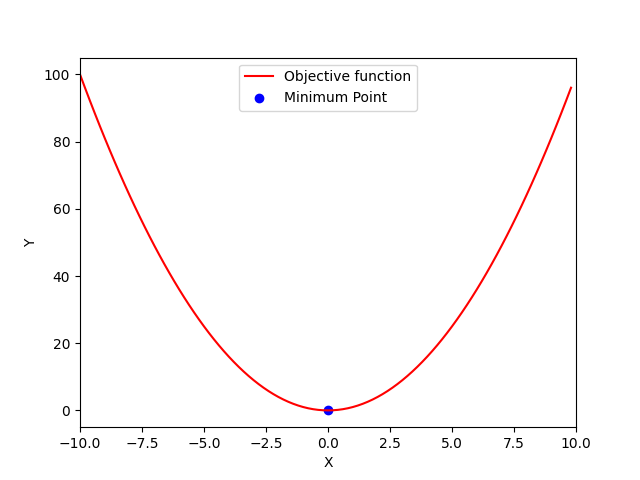
\includegraphics[width=0.7\columnwidth]{figs/fig.png}
    \caption{Minimum value of objective function}
\end{figure}
\end{document}  
